\csname if@print\endcsname
  % (print mode) skip online version front cover
\else
  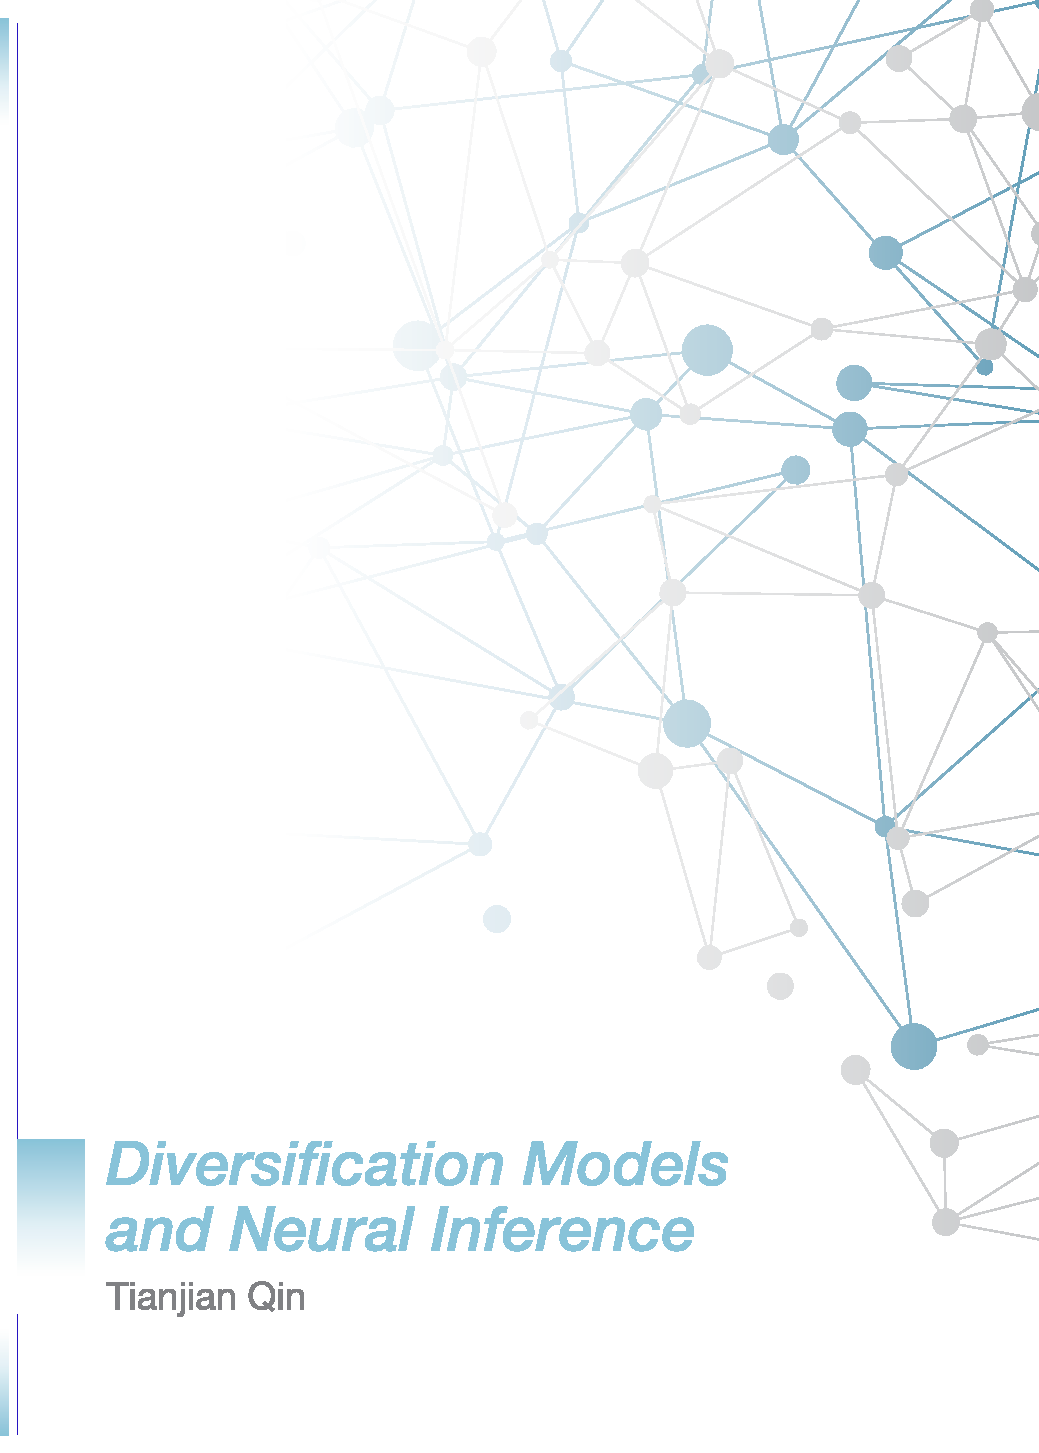
\includepdf[
    pages=1,
    fitpaper=true,
    pagecommand={\thispagestyle{empty}}
  ]{title/front-cover.pdf}
\fi

\begin{titlepage}
\thispagestyle{empty}

\begin{tikzpicture}[remember picture,overlay]
  \node[anchor=north] at ([yshift=-2.5cm]current page.north) {%
    
\includegraphics{title/logos/rug-en}%
  };
\end{tikzpicture}

\vspace*{3cm}

\begin{center}

\makeatletter
{\titlestyle\bfseries\LARGE\@title}
\makeatother

\makeatletter
\ifx\@subtitle\undefined\else
  \bigskip
  {\titlefont\titleshape\Large\@subtitle}
\fi
\makeatother

\vfill

{\Large\titlefont\bfseries PhD thesis}

\bigskip\bigskip

to obtain the degree of PhD of the

University of Groningen

on the authority of the

Rector Magnificus Prof.~J.M.A.~Scherpen

and in accordance with

the decision by the College of Deans.

This thesis will be defended in public on

Monday 4 May 2026 at 14.00 hours

\bigskip\bigskip

by

\bigskip\bigskip

\makeatletter
{\Large\titlefont\bfseries\@firstname\ \titleshape{\MakeUppercase{\@lastname}}}
\makeatother

\bigskip\bigskip

Master of Science in Wetland Ecology,

born on 5 January 1994.

\vspace*{2\bigskipamount}
\end{center}

\clearpage
\thispagestyle{empty}

\noindent This thesis has been approved by:

\medskip\noindent
\begin{tabular}{l}
    Supervisor: Prof. dr.\ R.S.\ Etienne \\
    Co-supervisor: Dr.\ L.L.\ Valente \\
    Co-supervisor: Dr.\ K.J.\ van Benthem
\end{tabular}

\bigskip
\noindent Assessment committee:

\begin{tabular}{p{4.5cm}l}
    Rector Magnificus, & chair \\
    Prof.\ dr.\ R.S.\ Etienne, & University of Groningen \\
    Dr.\ L.L.\ Valente, & Naturalis Biodiversity Center \\
    Dr.\ K.J.\ van Benthem, & University of Groningen \\

    \medskip
    \mbox{\emph{Independent members:}} & \\
    Prof.\ dr.\ E.C.\ Wit, & Università della Svizzera italiana \\
    Prof.\ dr.\ F.\ Hartig, & Universität Regensburg \\
    Prof.\ dr.\ S.\ Höhna, & Ludwig-Maximilians-Universität München \\
\end{tabular}

\medskip\medskip
\noindent This thesis was supported by the University of Groningen--China Scholarship Council joint scholarship program and carried out under the auspices of Groningen Institute for Evolutionary Life Sciences.

\medskip
\noindent
\begin{tabular}{@{}p{0.2\textwidth}@{}p{0.8\textwidth}}
  \textit{Keywords:} & macroevolution; diversity dependence; deep learning \\[\medskipamount]
  \textit{Printed by:} & HY Printing \\[\medskipamount]
  \textit{Cover:} & Tianjian Qin \\[\medskipamount]
  \textit{Style:} & Tianjian Qin, modified from Moritz Beller \\[\medskipamount]
\end{tabular}

\medskip\medskip
\noindent The author set this thesis in \LaTeX\xspace using the Libertinus, Inconsolata, and Noto CJK fonts.

\vspace{\bigskipamount}

\medskip
\noindent An electronic version of this thesis is available at \\
\url{https://github.com/EvoLandEco/Thesis/}.

\end{titlepage}

\begin{titlepage}
\thispagestyle{empty}

\begin{tikzpicture}[remember picture,overlay]
  \node[anchor=north] at ([yshift=-2.5cm]current page.north) {%
    \includegraphics{title/logos/rug}%
  };
\end{tikzpicture}

\vspace*{3cm}

\begin{center}

\makeatletter
{\titlestyle\bfseries\LARGE\@dutchtitle}
\makeatother

\makeatletter
\ifx\@dutchsubtitle\undefined\else
  \bigskip
  {\titlefont\titleshape\Large\@dutchsubtitle}
\fi
\makeatother

\vfill

{\Large\titlefont\bfseries Proefschrift}

\bigskip\bigskip

ter verkrijging van de graad van doctor aan de

Rijksuniversiteit Groningen

op gezag van de

rector magnificus prof.~dr.~ir.~J.M.A.~Scherpen

en volgens besluit van het College voor Promoties.

De openbare verdediging zal plaatsvinden op

maandag 4 mei 2026 om 14.00 uur

\bigskip\bigskip

door

\bigskip\bigskip

\makeatletter
{\Large\titlefont\bfseries\@firstname\ \titleshape{\MakeUppercase{\@lastname}}}
\makeatother

\bigskip\bigskip

Master of Science in Wetland Ecology,

geboren op 5 Januari 1994.

\vspace*{2\bigskipamount}
\end{center}

\clearpage
\thispagestyle{empty}

\noindent Dit proefschrift is goedgekeurd door de

\medskip\noindent
\begin{tabular}{l}
    promotor: Prof. dr.\ R.S.\ Etienne \\
    copromotor: Dr.\ L.L.\ Valente \\
    copromotor: Dr.\ K.J.\ van Benthem
\end{tabular}

\bigskip
\noindent Samenstelling promotiecommissie:

\begin{tabular}{p{4.5cm}l}
    Rector Magnificus, & voorzitter \\
    Prof.\ dr.\ R.S.\ Etienne, & Rijksuniversiteit Groningen \\
    Dr.\ L.L.\ Valente, & Naturalis Biodiversity Center \\
    Dr.\ K.J.\ van Benthem, & Rijksuniversiteit Groningen \\

    \medskip
    \mbox{\emph{Onafhankelijke leden:}} & \\
    Prof.\ dr.\ E.C.\ Wit, & Università della Svizzera italiana \\
    Prof.\ dr.\ F.\ Hartig, & Universität Regensburg \\
    Prof.\ dr.\ S.\ Höhna, & Ludwig-Maximilians-Universität München \\
\end{tabular}

\medskip\medskip
\noindent Dit proefschrift werd ondersteund door het gezamenlijke beursprogramma van de Rijksuniversiteit Groningen en de China Scholarship Council en uitgevoerd onder auspiciën van het Groningen Institute for Evolutionary Life Sciences.

\medskip
\noindent
\begin{tabular}{@{}p{0.2\textwidth}@{}p{0.8\textwidth}}
  \textit{Trefwoorden:} & macroevolutie; diversiteitsafhankelijkheid; deep learning \\[\medskipamount]
  \textit{Druk:} & HY Printing \\[\medskipamount]
  \textit{Omslag:} & Tianjian Qin \\[\medskipamount]
  \textit{Vormgeving:} & Tianjian Qin, aangepast van Moritz Beller \\[\medskipamount]
\end{tabular}

\medskip\medskip
\noindent De auteur zette dit proefschrift in \LaTeX\xspace met behulp van de Libertinus-, Inconsolata- en Noto CJK-lettertypen.

\vspace{\bigskipamount}

\medskip
\noindent Een elektronische versie van dit proefschrift is beschikbaar op \\
\url{https://github.com/EvoLandEco/Thesis/}.

\end{titlepage}
